\chapter{Calibration profile of the proposed model}\label{app:extra}
This appendix reports the calibration of the proposed model over the full
range of nominal coverage levels, as a complement to the single operating
point reported in the main line. Figure~\ref{fig:gp-reliability} sweeps the
nominal coverage from 10\% to 95\% and plots the empirical coverage against
it, on the development set and on the held-out test set. At the 90\%
operating point reported throughout, the model is close to nominal
(development 92.7\%, held-out test set \covGP). At central levels it is
conservative, with empirical coverage above nominal, and the PIT histograms
of Figure~\ref{fig:gp-pit} restate this as a mid-heavy shape: the predictive
distributions are somewhat wider in the tails than the realized errors. Two
properties of this profile bear on the hypotheses of the thesis. The profile
errs on the safe side, with intervals that are too wide rather than too
narrow, and it is indistinguishable between the development set and the
held-out test set. The calibration behaviour, unlike the pooled NLL
comparison of Table~\ref{tab:headline-conf}, therefore transfers to unseen
pieces unchanged. Further extended tables, namely the two-stage development
record, the $\mu=0$ block of the kernel study and the per-task detail of the
downstream evaluations, remain in the accompanying evidence archive rather
than in this appendix.

\begin{figure}[h]\centering
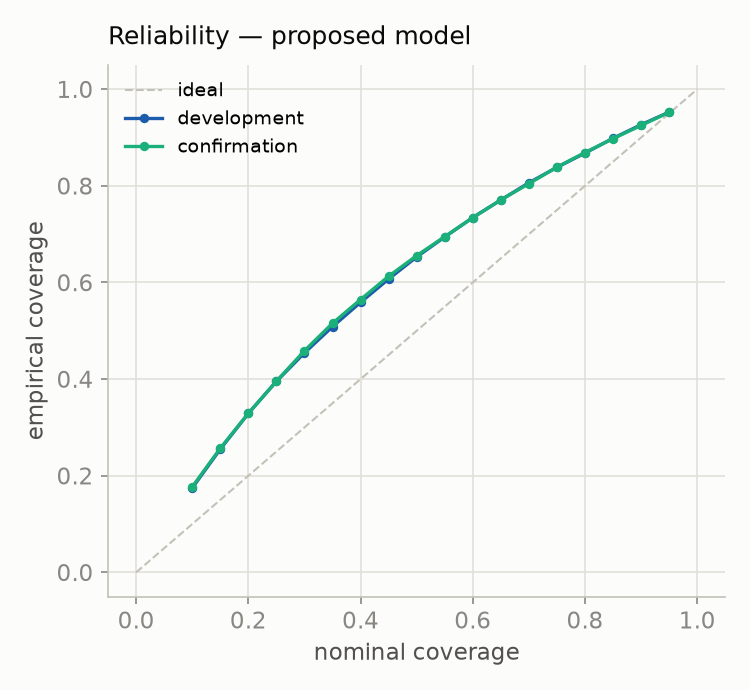
\includegraphics[width=0.62\linewidth]{figures/proposed_reliability.png}
\caption{Reliability diagram of the proposed model on the development set
and on the held-out test set.}
\label{fig:gp-reliability}
\end{figure}

\begin{figure}[h]\centering
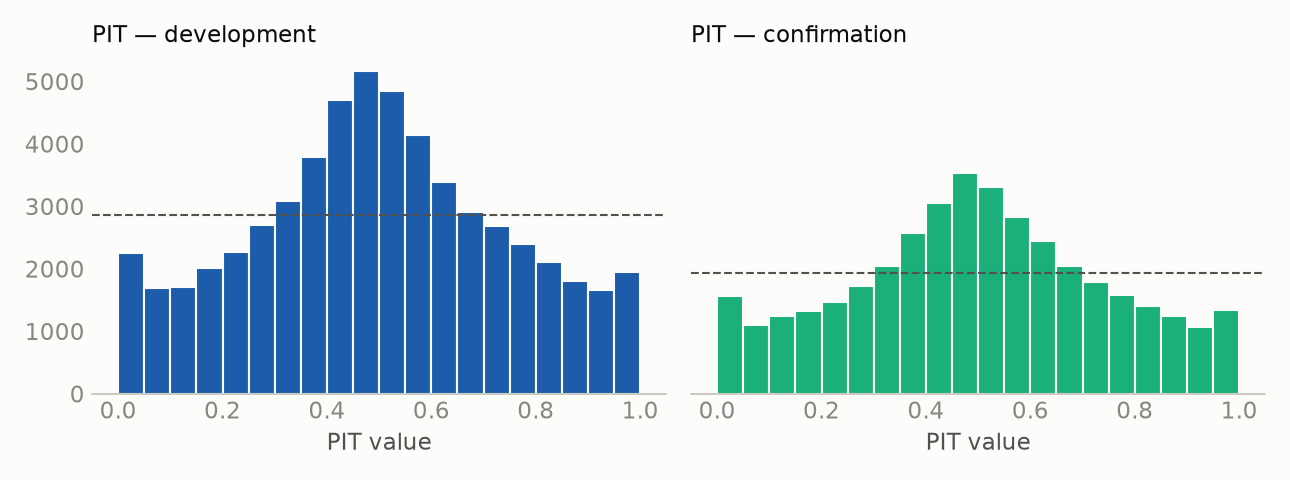
\includegraphics[width=0.9\linewidth]{figures/proposed_pit.png}
\caption{PIT histograms of the proposed model on the development set and on
the held-out test set. The dashed line is the uniform density.}
\label{fig:gp-pit}
\end{figure}

% =====================================================================
